\documentclass[a4paper, 11pt]{article}
\usepackage{fullpage, amssymb, amsmath, graphicx} 

\newcommand{\mytitle}{Problem Set 1}

\begin{document}
\noindent
\large\textbf{\mytitle} \\ \\ Tyler Gordon \\
\normalsize \today 
\ \ \hrulefill
All calculations can be found at github.com/tagordon/stars/hw1.ipynb
\section*{Problem 1}
	\subsection*{Part a}
		Using the relationship $M_\lambda = m_\lambda + 5 - 5\log(d)$, I find the absolute magnitude of 
		$\tau$ Sco to be $M_\lambda = -2.99$.
	\subsection*{Part b}
		Using the relationship $M_\text{bol} = -2.5\log(L/L_\odot) + 4.74$ and $M_\text{bol} = M_\text{v} + BC$, 
		I find the luminosity of $\tau$ Sco to be about $2.2\times10^4 L_\odot$.
	\subsection*{Part c}
		The flux from the star is related to the effective temperature by $F = \sigma T^4$, and the luminosity 
		is related to the star's radius by $L = 4\pi R^2F$. Solving for radius, we have:
		\begin{equation*}
			R = \sqrt{\frac{L}{4\pi\sigma T_\text{eff}^4}}
		\end{equation*}
		I find a radius of about $5.6 R_\odot$ for $\tau$ Sco. 
	\subsection*{Part d}
		Applying the mass luminosity relationship with the mean index $\alpha = 3.8$, I find that the mass of 
		$\tau$ Sco is about $14 M_\odot$.
	\subsection*{Part e}
		With the usual relations for surface gravity and escape velocity, I find $\log(g)=4.09$ and 
		$v_\text{esc}=1\times10^6 $ m/s. 
	\subsection*{Part f}
		The mean density of $\tau$ Sco is 0.11 g/cm$^{-3}$
	\subsection*{Part g}
		The sun has mean density 1.4 g/cm$^{-3}$, which is much larger than that fo $\tau$ Sco. It's surface 
		gravity is also larger ($\log(g)=4.44$), as expected for a more dense star, and it's escape velocity is 
		$6\times10^5$. The escape velocity is smaller because the sun is a less massive star that $\tau$ Sco. 
		
\section*{Problem 2}
	From the Virial Theorem, $K = -U/2$. For a self gravitating sphere of mass M and radius R, the potential energy 
	is $U = -GM^2/R$. For an ideal gas, the total kinetic energy is $K = 3Nk\bar{T}/2$. Where $N$, the total number of 
	particles, is $N = M/\mu m_H$. Plugging these expressions into the Virial Theorem:
	\begin{equation*}
		\frac{3}{2}\frac{M}{\mu m_H}k\bar{T} = \frac{GM^2}{2R}
	\end{equation*}
	Solving for the mean temperature $\bar{T}$, we find 
	\begin{equation*}
		\bar{T} = \frac{3\mu m_H}{k}\frac{GM}{R} \sim \frac{\mu m_H}{k}\frac{GM}{R}
	\end{equation*}
\section*{Problem 3}
	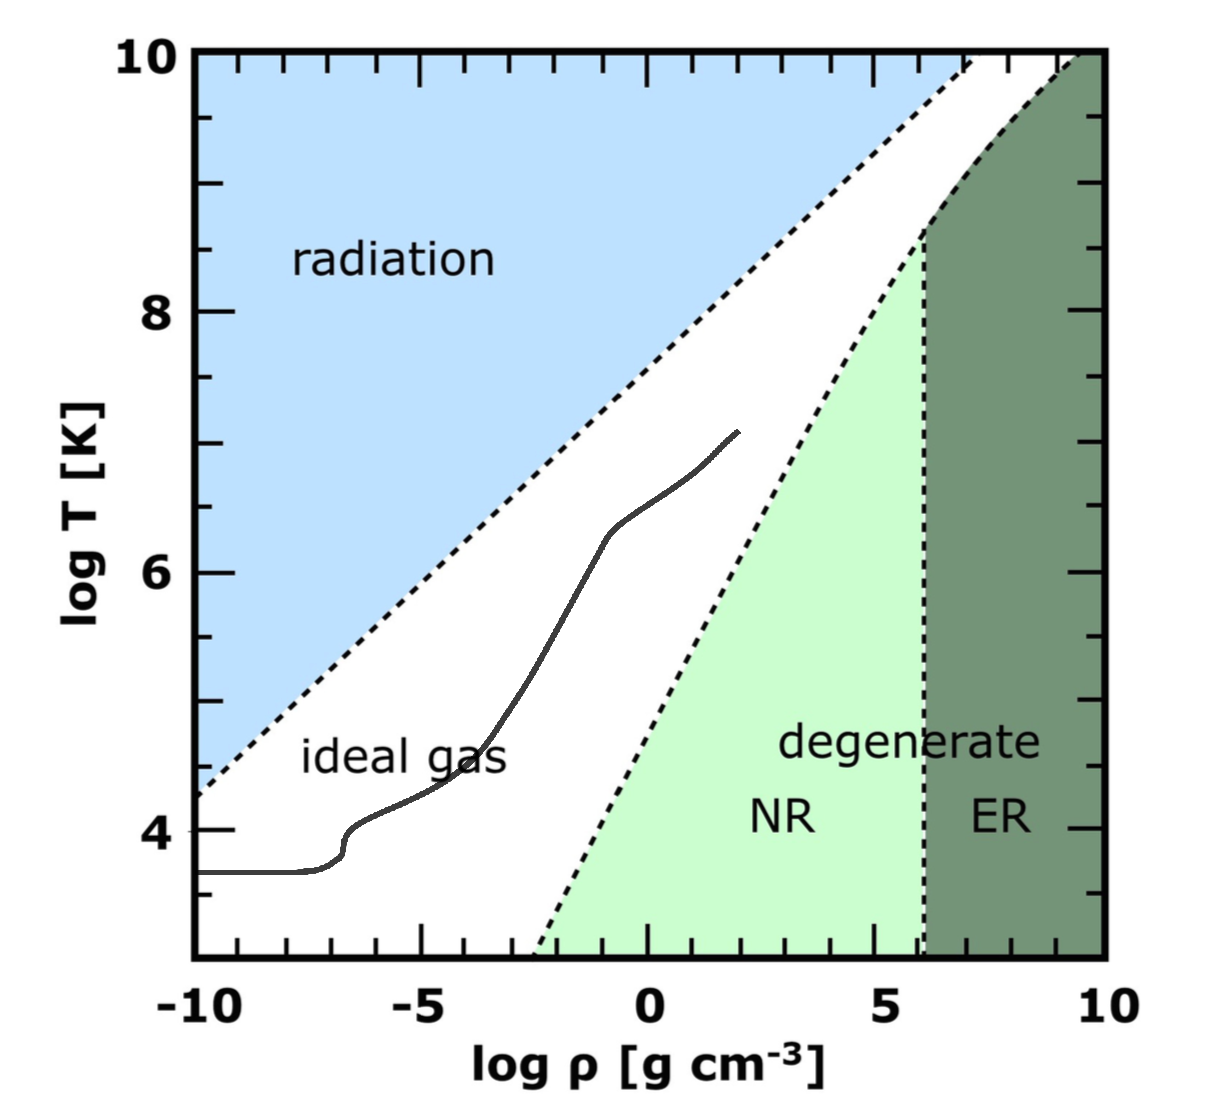
\includegraphics[width=15cm]{problem3.png}
	\ \\ \\
	From this plot we can conclude that the material making up the sun will behave as an ideal gas throughout the 
	entire star. 
\section*{Problem 4}
	\subsection*{Part a}
		Solving for N, the photon will undergo about $5\times10^{21}$ scatterings on it's way to the surface. 
	\subsection*{Part b}
		The total path length is thus $5\times10^{21}$ cm, and the time it takes to arrive at the surface would 
		be $5\times10^{21} \text{ cm}/3\times10^{10} \text{ cm/s} = 1.7\times10^{11}$ s
	\subsection*{Part c}
		No, scattering events change the energy of the photon. Changes in energy equate to changes in the 
		photon's wavelength. So it's a "different" photon by the time it reaches the surface. 
\section*{Problem 5}
	\subsection*{Part a}
		Fitting a power-law to the data from the appendix, I find the relation:
		\begin{equation*}
			\frac{L}{L_\odot} = 106\left(\frac{M}{M_\odot}\right)^{2.07}
		\end{equation*}
		\ \\ \\
		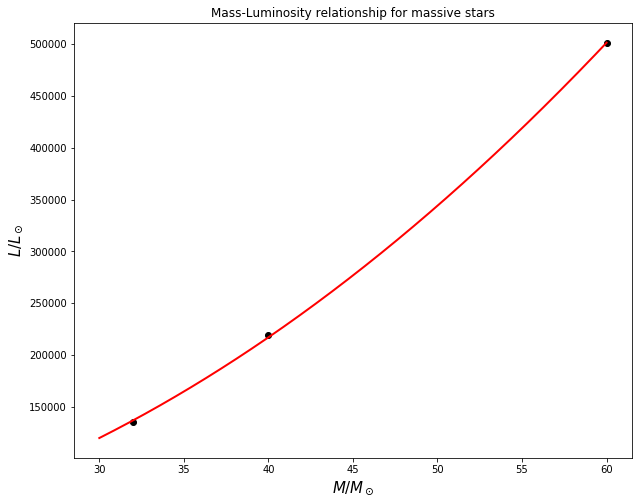
\includegraphics[width=15cm]{problem5.png}
		\ \\ \\
	\subsection*{Part b}
		Setting the right hand side equal to the Eddington Luminosity, the corresponding mass is found to be 
		about $M_\text{max} \sim 244 M_\odot$. 
\section*{Problem 6}
	\subsection*{Part a}
	The amount of energy that can be derived from the fuel in the core is given by:
	\begin{equation*}
		E = \chi M_\text{core}c^2
	\end{equation*}
	where $\chi$ is the efficiency of hydrogen fusion at converting mass to energy. To derive a timescale for 
	the main sequence evolution of the star we divide this by the star's luminosity. From figure 7.6 I estimate the 
	core mass-fraction of a $4 M_\odot$ star to be about $M_\text{core} = 0.2$, and for a $20 M_\odot$ star, 
	$M_\text{core} = 0.4$. The luminosities are given in the appendix as $log(L/L_\odot) = 2.37$ and $4.61$ 
	respectively. From these numbers (and adopting $\chi = 0.0071$ from section 8.1 of the book) I find 
	an approximate main sequence lifetime of 71 Myr for the $4 M_\odot$ star and about 8 Myr for the $20 M_\odot$ 
	star. 
	\subsection*{Part b}
		From appendix D, the $4 M_\odot$ star should have a main-sequence lifetime of about 151 Myr, and the 
		$20 M_\odot$ star should have a main-sequence lifetime of 7.7 Myr. Both of these are about correct to 
		an order of magnitude. I'm not sure why our assumptions give us a better estimate for the more massive star. 

\end{document}
